\subsection{Classes inherited from Robot class}
\label{concr:robot_classes}

In this chapter will be exposed classes which inherits
from \textit{Robot} class. They have to implement, at least,
the \textit{DrawRobot()} pure virtual father's method,
because \framework{} can not know in other way how to
represent the robot to overlap on the background image chosen.

\subsubsection{The Morduc Class}
\label{concr:robot_classes:concr:morduc}

This class allows to draw the robot when data and images
are retrieved from the log files created with the simulator
program (see chapter \ref{sec:simulator}).

\begin{figure}[!h]
  \begin{center}
    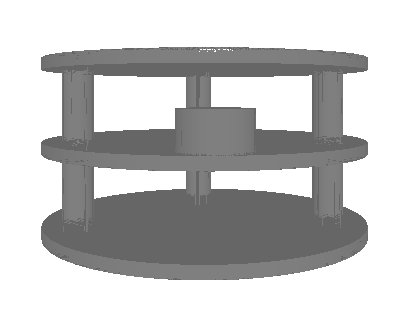
\includegraphics[width=200pt]{img/3morduc_opengl.png}
    \caption{Three dimensional model of Morduc}
    \label{fig:3morduc_opengl}
  \end{center}
\end{figure}

The \texttt{Morduc} class publicly inherits from \texttt{Robot} 
and, hence, implements the \texttt{DrawRobot()} method:

\begin{lstlisting}[caption={\texttt{Morduc} class declaration}, label={code:morducclass}, frame=trBL]
class Morduc : public Robot
{
 private:
  GLfloat radius;
  void PaintCylinder(GLfloat radius,GLfloat height);
  void PaintDisk(GLfloat radius);

 public:
  Morduc(float radius = 4.0f);
  void DrawRobot();
};
\end{lstlisting}

Such a method, reported in listing \ref{code:drawrobot}, contains the 
procedure to actually draw the OpenGL model representing Murdoc 
(in reality, Murdoc looks like a stack of three disks linked 
by thin cylinders - see figure \ref{fig:3morduc_opengl}).

\begin{lstlisting}[caption={\texttt{Morduc::DrawRobot()} function}, label={code:drawrobot}, frame=trBL]
void Morduc::DrawRobot()
{
  GLfloat reflectance_black[] = { 0.2f, 0.2f, 0.2f};
  GLfloat reflectance_white[] = { 0.8f, 0.8f, 0.8f};
  
  glMatrixMode(GL_MODELVIEW);  
  glPushMatrix();

  // set robot reflectance (it is black)
  glMaterialfv(GL_FRONT_AND_BACK, GL_AMBIENT, 
               reflectance_black);

  // set robot position
  glTranslatef(this -> x, 0.0f, this -> y);

  glRotatef(this -> theta, 0.0f, 1.0f, 0.0f);
  
  // translate on z axis
  // not to make the robot wipe the floor
  glTranslatef(0.0f,0.08f,0.0f);

  glScalef(radius, radius, radius);
  
  // draw robot
  PaintCylinder(1.0f, 0.1);
  PaintDisk(-1.0f);
  glTranslatef(0.0f, 0.1f, 0.0f);
  PaintDisk(1.0f);
  
  glTranslatef(0.0f, 0.6f, 0.0f);

  PaintCylinder(1.0f, 0.1f);
  PaintDisk(-1.0f);
  glTranslatef(0.0f, 0.1f, 0.0f);
  PaintDisk(1.0f);

  glTranslatef(0.8f, 0.0f, 0.0f);
  glColor3f(0.5f, 0.5f, 0.5f);
  PaintCylinder(0.2f, 0.3f);
  glTranslatef(0.0f, 0.3f, 0.0f);
  PaintDisk(0.2f);

  glTranslatef(0,0.401,0);
  glMaterialfv(GL_FRONT_AND_BACK, GL_AMBIENT, 
               reflectance_white);
  PaintDisk(0.1f);
  glTranslatef(0,-0.701,0);
  glMaterialfv(GL_FRONT_AND_BACK, GL_AMBIENT, 
               reflectance_black);

  glTranslatef(-0.8f, 0.0f, 0.0f);
  glColor3f(0.1f, 0.1f, 0.1f);
  glTranslatef(0.0f ,0.6f, 0.0f);
  PaintCylinder(1.0f, 0.1f);
  PaintDisk(-1.0f);
  glTranslatef(0.0f, 0.1f, 0.0f); 
  PaintDisk(1.0f);

  glTranslatef(0.0f, -1.5f, 0.0f);
  glTranslatef(0.0f, 0.0f, 0.8f);
  PaintCylinder(0.1f, 1.5f);
  glTranslatef(0.0f, 0.0f, -1.60f);
  PaintCylinder(0.1f, 1.5f);
  glTranslatef(-0.8f, 0.0f, 0.8f);

  PaintCylinder(0.1f, 1.5f);
  glTranslatef(0.8f, 0.0f, 0.0f);

  glScalef(1/radius, 1/radius, 1/radius);

  glPopMatrix();
}
\end{lstlisting}

Notice how such a function implements the skeleton 
presented in listing \ref{code:drawrobot_skeleton}.
\\
As you have surely noticed, \texttt{Morduc} contains also 
some private attributes, precisely two methods - 
\texttt{PaintCylinder()} and \texttt{PaintDisk()} - and 
a float field - \texttt{radius}.
\\
The two methods are just \textit{helper functions}, that is, 
functions that contains a procedure to draw, respectively,  
a \textit{disk} and a \textit{cylinder}.
\texttt{radius}, instead, stores the value of the radius 
for the of the cylinders which make up the robot.
After some calibration, the default \texttt{radius} value 
has been set to 4.0.
